\section{Results}

\subsection{Denaturation of dsDNA}

It has long been known that double stranded DNA (in our case, the characteristic double helix of B-DNA) exists in circumstances with temperatures $<$ (330--360)K, with the precise `melting' point (where dsDNA denaturates to single stranded DNA) depending on the basepair configuration, the length of the strand and the salt concentration in the environment. When the temperature is raised to or above this critical point, the basepair bonding potential no longer dominates the increasing kinetic energy of the system and the two strands separate. 

This `unwinding' of double stranded DNA is a very complex process because of the inherent helical structure of a DNA double helix. Simple `zipper' mechanisms are not enough to simulate this behavior because local changes to the system (i.e. the unzipping of one complementary basepair) have a global effect (twisting the rest of the strand) (see Baiesi \etal, \cite{carlon2010unwinding}). Before we discuss more quantitative elements of this behavior, we first reproduce some basic predictions of the original Knotts \etal\ model \cite{knotts2007coarse} to illustrate this unwinding effect.

\paragraph{Knotts III.A.1: 5'-GCGTCATACAGTGC-3'} To demonstrate the simple denaturation of a short strand of dsDNA, we simulated the behaviour of a double helix configuration 5'-GCGTCATACAGTGC-3' (14 basepairs) to check if the time-evolution is as expected from the same simulation in the paper of Knotts \etal \cite{knotts2007coarse}. We find that the melting temperature of this configuration lies around 335-340K; with a salt concentration of 50 mM our results agree with the simulations of Knotts. In Figure \ref{knotts1_configs} and Figure \ref{knotts1_lines} the basepair configurations are illustrated.

\begin{figure}[h] \begin{minipage}{7cm}
-e                \scalebox{0.8}{
                        \nonstopmode
                        % GNUPLOT: LaTeX picture with Postscript
\begingroup
  \makeatletter
  \providecommand\color[2][]{%
    \GenericError{(gnuplot) \space\space\space\@spaces}{%
      Package color not loaded in conjunction with
      terminal option `colourtext'%
    }{See the gnuplot documentation for explanation.%
    }{Either use 'blacktext' in gnuplot or load the package
      color.sty in LaTeX.}%
    \renewcommand\color[2][]{}%
  }%
  \providecommand\includegraphics[2][]{%
    \GenericError{(gnuplot) \space\space\space\@spaces}{%
      Package graphicx or graphics not loaded%
    }{See the gnuplot documentation for explanation.%
    }{The gnuplot epslatex terminal needs graphicx.sty or graphics.sty.}%
    \renewcommand\includegraphics[2][]{}%
  }%
  \providecommand\rotatebox[2]{#2}%
  \@ifundefined{ifGPcolor}{%
    \newif\ifGPcolor
    \GPcolortrue
  }{}%
  \@ifundefined{ifGPblacktext}{%
    \newif\ifGPblacktext
    \GPblacktexttrue
  }{}%
  % define a \g@addto@macro without @ in the name:
  \let\gplgaddtomacro\g@addto@macro
  % define empty templates for all commands taking text:
  \gdef\gplbacktext{}%
  \gdef\gplfronttext{}%
  \makeatother
  \ifGPblacktext
    % no textcolor at all
    \def\colorrgb#1{}%
    \def\colorgray#1{}%
  \else
    % gray or color?
    \ifGPcolor
      \def\colorrgb#1{\color[rgb]{#1}}%
      \def\colorgray#1{\color[gray]{#1}}%
      \expandafter\def\csname LTw\endcsname{\color{white}}%
      \expandafter\def\csname LTb\endcsname{\color{black}}%
      \expandafter\def\csname LTa\endcsname{\color{black}}%
      \expandafter\def\csname LT0\endcsname{\color[rgb]{1,0,0}}%
      \expandafter\def\csname LT1\endcsname{\color[rgb]{0,1,0}}%
      \expandafter\def\csname LT2\endcsname{\color[rgb]{0,0,1}}%
      \expandafter\def\csname LT3\endcsname{\color[rgb]{1,0,1}}%
      \expandafter\def\csname LT4\endcsname{\color[rgb]{0,1,1}}%
      \expandafter\def\csname LT5\endcsname{\color[rgb]{1,1,0}}%
      \expandafter\def\csname LT6\endcsname{\color[rgb]{0,0,0}}%
      \expandafter\def\csname LT7\endcsname{\color[rgb]{1,0.3,0}}%
      \expandafter\def\csname LT8\endcsname{\color[rgb]{0.5,0.5,0.5}}%
    \else
      % gray
      \def\colorrgb#1{\color{black}}%
      \def\colorgray#1{\color[gray]{#1}}%
      \expandafter\def\csname LTw\endcsname{\color{white}}%
      \expandafter\def\csname LTb\endcsname{\color{black}}%
      \expandafter\def\csname LTa\endcsname{\color{black}}%
      \expandafter\def\csname LT0\endcsname{\color{black}}%
      \expandafter\def\csname LT1\endcsname{\color{black}}%
      \expandafter\def\csname LT2\endcsname{\color{black}}%
      \expandafter\def\csname LT3\endcsname{\color{black}}%
      \expandafter\def\csname LT4\endcsname{\color{black}}%
      \expandafter\def\csname LT5\endcsname{\color{black}}%
      \expandafter\def\csname LT6\endcsname{\color{black}}%
      \expandafter\def\csname LT7\endcsname{\color{black}}%
      \expandafter\def\csname LT8\endcsname{\color{black}}%
    \fi
  \fi
  \setlength{\unitlength}{0.0500bp}%
  \begin{picture}(5760.00,3840.00)%
    \gplgaddtomacro\gplbacktext{%
      \colorrgb{0.00,0.00,0.00}%
      \put(110,1986){\rotatebox{90}{\makebox(0,0){\strut{}\rule{0pt}{-1.5cm}}}}%
    }%
    \gplgaddtomacro\gplfronttext{%
      \colorrgb{0.00,0.00,0.00}%
      \put(616,3310){\makebox(0,0)[r]{\strut{}2}}%
      \colorrgb{0.00,0.00,0.00}%
      \put(616,2829){\makebox(0,0)[r]{\strut{}4}}%
      \colorrgb{0.00,0.00,0.00}%
      \put(616,2348){\makebox(0,0)[r]{\strut{}6}}%
      \colorrgb{0.00,0.00,0.00}%
      \put(616,1866){\makebox(0,0)[r]{\strut{}8}}%
      \colorrgb{0.00,0.00,0.00}%
      \put(616,1385){\makebox(0,0)[r]{\strut{}10}}%
      \colorrgb{0.00,0.00,0.00}%
      \put(616,903){\makebox(0,0)[r]{\strut{}12}}%
      \colorrgb{0.00,0.00,0.00}%
      \put(616,422){\makebox(0,0)[r]{\strut{}14}}%
      \colorrgb{0.00,0.00,0.00}%
      \put(748,202){\makebox(0,0){\strut{}0}}%
      \colorrgb{0.00,0.00,0.00}%
      \put(1305,202){\makebox(0,0){\strut{}1e-08}}%
      \colorrgb{0.00,0.00,0.00}%
      \put(1863,202){\makebox(0,0){\strut{}2e-08}}%
      \colorrgb{0.00,0.00,0.00}%
      \put(2420,202){\makebox(0,0){\strut{}3e-08}}%
      \colorrgb{0.00,0.00,0.00}%
      \put(2977,202){\makebox(0,0){\strut{}4e-08}}%
      \colorrgb{0.00,0.00,0.00}%
      \put(3535,202){\makebox(0,0){\strut{}5e-08}}%
      \colorrgb{0.00,0.00,0.00}%
      \put(4092,202){\makebox(0,0){\strut{}6e-08}}%
      \colorrgb{0.00,0.00,0.00}%
      \put(4649,202){\makebox(0,0){\strut{}7e-08}}%
      \colorrgb{0.00,0.00,0.00}%
      \put(5206,202){\makebox(0,0){\strut{}8e-08}}%
    }%
    \gplbacktext
    \put(0,0){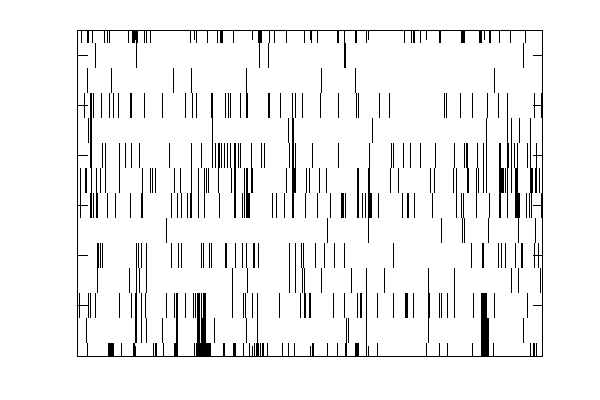
\includegraphics{images/data_knotts1/knotts1_T330}}%
    \gplfronttext
  \end{picture}%
\endgroup

                        \errorstopmode
                        \rule[-0.5cm]{0cm}{0cm}}
 \end{minipage} \begin{minipage}{7cm} -e                \scalebox{0.8}{
                        \nonstopmode
                        % GNUPLOT: LaTeX picture with Postscript
\begingroup
  \makeatletter
  \providecommand\color[2][]{%
    \GenericError{(gnuplot) \space\space\space\@spaces}{%
      Package color not loaded in conjunction with
      terminal option `colourtext'%
    }{See the gnuplot documentation for explanation.%
    }{Either use 'blacktext' in gnuplot or load the package
      color.sty in LaTeX.}%
    \renewcommand\color[2][]{}%
  }%
  \providecommand\includegraphics[2][]{%
    \GenericError{(gnuplot) \space\space\space\@spaces}{%
      Package graphicx or graphics not loaded%
    }{See the gnuplot documentation for explanation.%
    }{The gnuplot epslatex terminal needs graphicx.sty or graphics.sty.}%
    \renewcommand\includegraphics[2][]{}%
  }%
  \providecommand\rotatebox[2]{#2}%
  \@ifundefined{ifGPcolor}{%
    \newif\ifGPcolor
    \GPcolortrue
  }{}%
  \@ifundefined{ifGPblacktext}{%
    \newif\ifGPblacktext
    \GPblacktexttrue
  }{}%
  % define a \g@addto@macro without @ in the name:
  \let\gplgaddtomacro\g@addto@macro
  % define empty templates for all commands taking text:
  \gdef\gplbacktext{}%
  \gdef\gplfronttext{}%
  \makeatother
  \ifGPblacktext
    % no textcolor at all
    \def\colorrgb#1{}%
    \def\colorgray#1{}%
  \else
    % gray or color?
    \ifGPcolor
      \def\colorrgb#1{\color[rgb]{#1}}%
      \def\colorgray#1{\color[gray]{#1}}%
      \expandafter\def\csname LTw\endcsname{\color{white}}%
      \expandafter\def\csname LTb\endcsname{\color{black}}%
      \expandafter\def\csname LTa\endcsname{\color{black}}%
      \expandafter\def\csname LT0\endcsname{\color[rgb]{1,0,0}}%
      \expandafter\def\csname LT1\endcsname{\color[rgb]{0,1,0}}%
      \expandafter\def\csname LT2\endcsname{\color[rgb]{0,0,1}}%
      \expandafter\def\csname LT3\endcsname{\color[rgb]{1,0,1}}%
      \expandafter\def\csname LT4\endcsname{\color[rgb]{0,1,1}}%
      \expandafter\def\csname LT5\endcsname{\color[rgb]{1,1,0}}%
      \expandafter\def\csname LT6\endcsname{\color[rgb]{0,0,0}}%
      \expandafter\def\csname LT7\endcsname{\color[rgb]{1,0.3,0}}%
      \expandafter\def\csname LT8\endcsname{\color[rgb]{0.5,0.5,0.5}}%
    \else
      % gray
      \def\colorrgb#1{\color{black}}%
      \def\colorgray#1{\color[gray]{#1}}%
      \expandafter\def\csname LTw\endcsname{\color{white}}%
      \expandafter\def\csname LTb\endcsname{\color{black}}%
      \expandafter\def\csname LTa\endcsname{\color{black}}%
      \expandafter\def\csname LT0\endcsname{\color{black}}%
      \expandafter\def\csname LT1\endcsname{\color{black}}%
      \expandafter\def\csname LT2\endcsname{\color{black}}%
      \expandafter\def\csname LT3\endcsname{\color{black}}%
      \expandafter\def\csname LT4\endcsname{\color{black}}%
      \expandafter\def\csname LT5\endcsname{\color{black}}%
      \expandafter\def\csname LT6\endcsname{\color{black}}%
      \expandafter\def\csname LT7\endcsname{\color{black}}%
      \expandafter\def\csname LT8\endcsname{\color{black}}%
    \fi
  \fi
  \setlength{\unitlength}{0.0500bp}%
  \begin{picture}(5760.00,3840.00)%
    \gplgaddtomacro\gplbacktext{%
      \colorrgb{0.00,0.00,0.00}%
      \put(110,1986){\rotatebox{90}{\makebox(0,0){\strut{}\rule{0pt}{-1.5cm}}}}%
    }%
    \gplgaddtomacro\gplfronttext{%
      \colorrgb{0.00,0.00,0.00}%
      \put(616,3310){\makebox(0,0)[r]{\strut{}2}}%
      \colorrgb{0.00,0.00,0.00}%
      \put(616,2829){\makebox(0,0)[r]{\strut{}4}}%
      \colorrgb{0.00,0.00,0.00}%
      \put(616,2348){\makebox(0,0)[r]{\strut{}6}}%
      \colorrgb{0.00,0.00,0.00}%
      \put(616,1866){\makebox(0,0)[r]{\strut{}8}}%
      \colorrgb{0.00,0.00,0.00}%
      \put(616,1385){\makebox(0,0)[r]{\strut{}10}}%
      \colorrgb{0.00,0.00,0.00}%
      \put(616,903){\makebox(0,0)[r]{\strut{}12}}%
      \colorrgb{0.00,0.00,0.00}%
      \put(616,422){\makebox(0,0)[r]{\strut{}14}}%
      \colorrgb{0.00,0.00,0.00}%
      \put(748,202){\makebox(0,0){\strut{}0}}%
      \colorrgb{0.00,0.00,0.00}%
      \put(1305,202){\makebox(0,0){\strut{}100}}%
      \colorrgb{0.00,0.00,0.00}%
      \put(1863,202){\makebox(0,0){\strut{}200}}%
      \colorrgb{0.00,0.00,0.00}%
      \put(2420,202){\makebox(0,0){\strut{}300}}%
      \colorrgb{0.00,0.00,0.00}%
      \put(2977,202){\makebox(0,0){\strut{}400}}%
      \colorrgb{0.00,0.00,0.00}%
      \put(3535,202){\makebox(0,0){\strut{}500}}%
      \colorrgb{0.00,0.00,0.00}%
      \put(4092,202){\makebox(0,0){\strut{}600}}%
      \colorrgb{0.00,0.00,0.00}%
      \put(4649,202){\makebox(0,0){\strut{}700}}%
      \colorrgb{0.00,0.00,0.00}%
      \put(5206,202){\makebox(0,0){\strut{}800}}%
    }%
    \gplbacktext
    \put(0,0){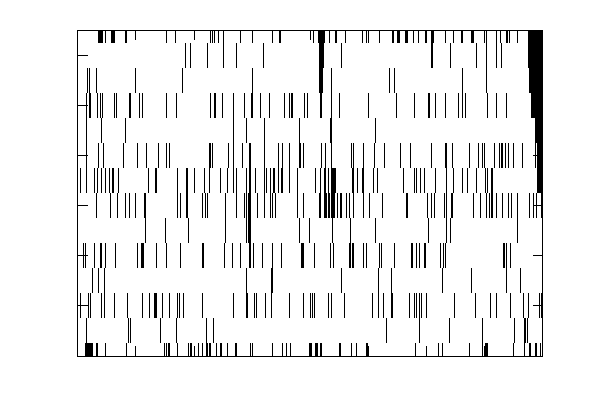
\includegraphics{images//data_knotts1/knotts1_T335}}%
    \gplfronttext
  \end{picture}%
\endgroup

                        \errorstopmode
                        \rule[-0.5cm]{0cm}{0cm}}
 \end{minipage}
\begin{minipage}{7cm}
\begin{figure}[htb]
       \begin{center}
               \scalebox{0.5}{
                        \nonstopmode
                        % GNUPLOT: LaTeX picture with Postscript
\begingroup
  \makeatletter
  \providecommand\color[2][]{%
    \GenericError{(gnuplot) \space\space\space\@spaces}{%
      Package color not loaded in conjunction with
      terminal option `colourtext'%
    }{See the gnuplot documentation for explanation.%
    }{Either use 'blacktext' in gnuplot or load the package
      color.sty in LaTeX.}%
    \renewcommand\color[2][]{}%
  }%
  \providecommand\includegraphics[2][]{%
    \GenericError{(gnuplot) \space\space\space\@spaces}{%
      Package graphicx or graphics not loaded%
    }{See the gnuplot documentation for explanation.%
    }{The gnuplot epslatex terminal needs graphicx.sty or graphics.sty.}%
    \renewcommand\includegraphics[2][]{}%
  }%
  \providecommand\rotatebox[2]{#2}%
  \@ifundefined{ifGPcolor}{%
    \newif\ifGPcolor
    \GPcolortrue
  }{}%
  \@ifundefined{ifGPblacktext}{%
    \newif\ifGPblacktext
    \GPblacktexttrue
  }{}%
  % define a \g@addto@macro without @ in the name:
  \let\gplgaddtomacro\g@addto@macro
  % define empty templates for all commands taking text:
  \gdef\gplbacktext{}%
  \gdef\gplfronttext{}%
  \makeatother
  \ifGPblacktext
    % no textcolor at all
    \def\colorrgb#1{}%
    \def\colorgray#1{}%
  \else
    % gray or color?
    \ifGPcolor
      \def\colorrgb#1{\color[rgb]{#1}}%
      \def\colorgray#1{\color[gray]{#1}}%
      \expandafter\def\csname LTw\endcsname{\color{white}}%
      \expandafter\def\csname LTb\endcsname{\color{black}}%
      \expandafter\def\csname LTa\endcsname{\color{black}}%
      \expandafter\def\csname LT0\endcsname{\color[rgb]{1,0,0}}%
      \expandafter\def\csname LT1\endcsname{\color[rgb]{0,1,0}}%
      \expandafter\def\csname LT2\endcsname{\color[rgb]{0,0,1}}%
      \expandafter\def\csname LT3\endcsname{\color[rgb]{1,0,1}}%
      \expandafter\def\csname LT4\endcsname{\color[rgb]{0,1,1}}%
      \expandafter\def\csname LT5\endcsname{\color[rgb]{1,1,0}}%
      \expandafter\def\csname LT6\endcsname{\color[rgb]{0,0,0}}%
      \expandafter\def\csname LT7\endcsname{\color[rgb]{1,0.3,0}}%
      \expandafter\def\csname LT8\endcsname{\color[rgb]{0.5,0.5,0.5}}%
    \else
      % gray
      \def\colorrgb#1{\color{black}}%
      \def\colorgray#1{\color[gray]{#1}}%
      \expandafter\def\csname LTw\endcsname{\color{white}}%
      \expandafter\def\csname LTb\endcsname{\color{black}}%
      \expandafter\def\csname LTa\endcsname{\color{black}}%
      \expandafter\def\csname LT0\endcsname{\color{black}}%
      \expandafter\def\csname LT1\endcsname{\color{black}}%
      \expandafter\def\csname LT2\endcsname{\color{black}}%
      \expandafter\def\csname LT3\endcsname{\color{black}}%
      \expandafter\def\csname LT4\endcsname{\color{black}}%
      \expandafter\def\csname LT5\endcsname{\color{black}}%
      \expandafter\def\csname LT6\endcsname{\color{black}}%
      \expandafter\def\csname LT7\endcsname{\color{black}}%
      \expandafter\def\csname LT8\endcsname{\color{black}}%
    \fi
  \fi
  \setlength{\unitlength}{0.0500bp}%
  \begin{picture}(5760.00,3840.00)%
    \gplgaddtomacro\gplbacktext{%
      \colorrgb{0.00,0.00,0.00}%
      \put(110,1986){\rotatebox{90}{\makebox(0,0){\strut{}\rule{0pt}{-1.5cm}}}}%
    }%
    \gplgaddtomacro\gplfronttext{%
      \colorrgb{0.00,0.00,0.00}%
      \put(616,3310){\makebox(0,0)[r]{\strut{}2}}%
      \colorrgb{0.00,0.00,0.00}%
      \put(616,2829){\makebox(0,0)[r]{\strut{}4}}%
      \colorrgb{0.00,0.00,0.00}%
      \put(616,2348){\makebox(0,0)[r]{\strut{}6}}%
      \colorrgb{0.00,0.00,0.00}%
      \put(616,1866){\makebox(0,0)[r]{\strut{}8}}%
      \colorrgb{0.00,0.00,0.00}%
      \put(616,1385){\makebox(0,0)[r]{\strut{}10}}%
      \colorrgb{0.00,0.00,0.00}%
      \put(616,903){\makebox(0,0)[r]{\strut{}12}}%
      \colorrgb{0.00,0.00,0.00}%
      \put(616,422){\makebox(0,0)[r]{\strut{}14}}%
      \colorrgb{0.00,0.00,0.00}%
      \put(748,202){\makebox(0,0){\strut{}0}}%
      \colorrgb{0.00,0.00,0.00}%
      \put(1305,202){\makebox(0,0){\strut{}10}}%
      \colorrgb{0.00,0.00,0.00}%
      \put(1863,202){\makebox(0,0){\strut{}20}}%
      \colorrgb{0.00,0.00,0.00}%
      \put(2420,202){\makebox(0,0){\strut{}30}}%
      \colorrgb{0.00,0.00,0.00}%
      \put(2977,202){\makebox(0,0){\strut{}40}}%
      \colorrgb{0.00,0.00,0.00}%
      \put(3535,202){\makebox(0,0){\strut{}50}}%
      \colorrgb{0.00,0.00,0.00}%
      \put(4092,202){\makebox(0,0){\strut{}60}}%
      \colorrgb{0.00,0.00,0.00}%
      \put(4649,202){\makebox(0,0){\strut{}70}}%
      \colorrgb{0.00,0.00,0.00}%
      \put(5206,202){\makebox(0,0){\strut{}80}}%
    }%
    \gplbacktext
    \put(0,0){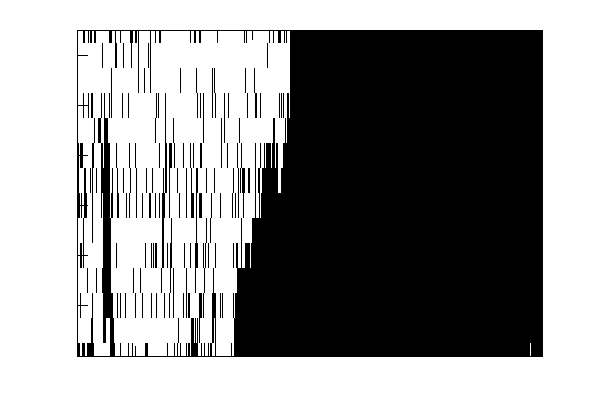
\includegraphics{images//data_knotts1/knotts1_T350}}%
    \gplfronttext
  \end{picture}%
\endgroup

                        \errorstopmode
                        \rule[-0.5cm]{0cm}{0cm}}
                \caption{}
                \label{data_knotts1/knotts1_T350}
        \end{center}
\end{figure}

 \end{minipage} \begin{minipage}{7cm}
               \scalebox{0.5}{
                        \nonstopmode
                        % GNUPLOT: LaTeX picture with Postscript
\begingroup
  \makeatletter
  \providecommand\color[2][]{%
    \GenericError{(gnuplot) \space\space\space\@spaces}{%
      Package color not loaded in conjunction with
      terminal option `colourtext'%
    }{See the gnuplot documentation for explanation.%
    }{Either use 'blacktext' in gnuplot or load the package
      color.sty in LaTeX.}%
    \renewcommand\color[2][]{}%
  }%
  \providecommand\includegraphics[2][]{%
    \GenericError{(gnuplot) \space\space\space\@spaces}{%
      Package graphicx or graphics not loaded%
    }{See the gnuplot documentation for explanation.%
    }{The gnuplot epslatex terminal needs graphicx.sty or graphics.sty.}%
    \renewcommand\includegraphics[2][]{}%
  }%
  \providecommand\rotatebox[2]{#2}%
  \@ifundefined{ifGPcolor}{%
    \newif\ifGPcolor
    \GPcolortrue
  }{}%
  \@ifundefined{ifGPblacktext}{%
    \newif\ifGPblacktext
    \GPblacktexttrue
  }{}%
  % define a \g@addto@macro without @ in the name:
  \let\gplgaddtomacro\g@addto@macro
  % define empty templates for all commands taking text:
  \gdef\gplbacktext{}%
  \gdef\gplfronttext{}%
  \makeatother
  \ifGPblacktext
    % no textcolor at all
    \def\colorrgb#1{}%
    \def\colorgray#1{}%
  \else
    % gray or color?
    \ifGPcolor
      \def\colorrgb#1{\color[rgb]{#1}}%
      \def\colorgray#1{\color[gray]{#1}}%
      \expandafter\def\csname LTw\endcsname{\color{white}}%
      \expandafter\def\csname LTb\endcsname{\color{black}}%
      \expandafter\def\csname LTa\endcsname{\color{black}}%
      \expandafter\def\csname LT0\endcsname{\color[rgb]{1,0,0}}%
      \expandafter\def\csname LT1\endcsname{\color[rgb]{0,1,0}}%
      \expandafter\def\csname LT2\endcsname{\color[rgb]{0,0,1}}%
      \expandafter\def\csname LT3\endcsname{\color[rgb]{1,0,1}}%
      \expandafter\def\csname LT4\endcsname{\color[rgb]{0,1,1}}%
      \expandafter\def\csname LT5\endcsname{\color[rgb]{1,1,0}}%
      \expandafter\def\csname LT6\endcsname{\color[rgb]{0,0,0}}%
      \expandafter\def\csname LT7\endcsname{\color[rgb]{1,0.3,0}}%
      \expandafter\def\csname LT8\endcsname{\color[rgb]{0.5,0.5,0.5}}%
    \else
      % gray
      \def\colorrgb#1{\color{black}}%
      \def\colorgray#1{\color[gray]{#1}}%
      \expandafter\def\csname LTw\endcsname{\color{white}}%
      \expandafter\def\csname LTb\endcsname{\color{black}}%
      \expandafter\def\csname LTa\endcsname{\color{black}}%
      \expandafter\def\csname LT0\endcsname{\color{black}}%
      \expandafter\def\csname LT1\endcsname{\color{black}}%
      \expandafter\def\csname LT2\endcsname{\color{black}}%
      \expandafter\def\csname LT3\endcsname{\color{black}}%
      \expandafter\def\csname LT4\endcsname{\color{black}}%
      \expandafter\def\csname LT5\endcsname{\color{black}}%
      \expandafter\def\csname LT6\endcsname{\color{black}}%
      \expandafter\def\csname LT7\endcsname{\color{black}}%
      \expandafter\def\csname LT8\endcsname{\color{black}}%
    \fi
  \fi
  \setlength{\unitlength}{0.0500bp}%
  \begin{picture}(5760.00,3840.00)%
    \gplgaddtomacro\gplbacktext{%
      \colorrgb{0.00,0.00,0.00}%
      \put(110,1986){\rotatebox{90}{\makebox(0,0){\strut{}\rule{0pt}{-1.5cm}}}}%
    }%
    \gplgaddtomacro\gplfronttext{%
      \colorrgb{0.00,0.00,0.00}%
      \put(616,3310){\makebox(0,0)[r]{\strut{}2}}%
      \colorrgb{0.00,0.00,0.00}%
      \put(616,2829){\makebox(0,0)[r]{\strut{}4}}%
      \colorrgb{0.00,0.00,0.00}%
      \put(616,2348){\makebox(0,0)[r]{\strut{}6}}%
      \colorrgb{0.00,0.00,0.00}%
      \put(616,1866){\makebox(0,0)[r]{\strut{}8}}%
      \colorrgb{0.00,0.00,0.00}%
      \put(616,1385){\makebox(0,0)[r]{\strut{}10}}%
      \colorrgb{0.00,0.00,0.00}%
      \put(616,903){\makebox(0,0)[r]{\strut{}12}}%
      \colorrgb{0.00,0.00,0.00}%
      \put(616,422){\makebox(0,0)[r]{\strut{}14}}%
      \colorrgb{0.00,0.00,0.00}%
      \put(748,202){\makebox(0,0){\strut{}0}}%
      \colorrgb{0.00,0.00,0.00}%
      \put(1305,202){\makebox(0,0){\strut{}1e-08}}%
      \colorrgb{0.00,0.00,0.00}%
      \put(1863,202){\makebox(0,0){\strut{}2e-08}}%
      \colorrgb{0.00,0.00,0.00}%
      \put(2420,202){\makebox(0,0){\strut{}3e-08}}%
      \colorrgb{0.00,0.00,0.00}%
      \put(2977,202){\makebox(0,0){\strut{}4e-08}}%
      \colorrgb{0.00,0.00,0.00}%
      \put(3535,202){\makebox(0,0){\strut{}5e-08}}%
      \colorrgb{0.00,0.00,0.00}%
      \put(4092,202){\makebox(0,0){\strut{}6e-08}}%
      \colorrgb{0.00,0.00,0.00}%
      \put(4649,202){\makebox(0,0){\strut{}7e-08}}%
      \colorrgb{0.00,0.00,0.00}%
      \put(5206,202){\makebox(0,0){\strut{}8e-08}}%
    }%
    \gplbacktext
    \put(0,0){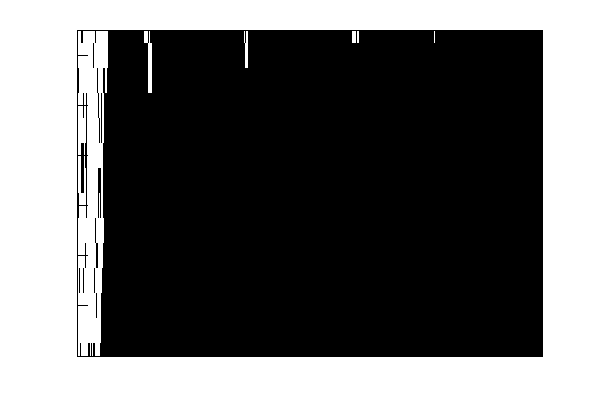
\includegraphics{images/knotts1_T360}}%
    \gplfronttext
  \end{picture}%
\endgroup

                        \errorstopmode
                        \rule[-0.5cm]{0cm}{0cm}}


\end{minipage}\begin{center}
 \scalebox{0.8}{
                        \nonstopmode
                        % GNUPLOT: LaTeX picture with Postscript
\begingroup
  \makeatletter
  \providecommand\color[2][]{%
    \GenericError{(gnuplot) \space\space\space\@spaces}{%
      Package color not loaded in conjunction with
      terminal option `colourtext'%
    }{See the gnuplot documentation for explanation.%
    }{Either use 'blacktext' in gnuplot or load the package
      color.sty in LaTeX.}%
    \renewcommand\color[2][]{}%
  }%
  \providecommand\includegraphics[2][]{%
    \GenericError{(gnuplot) \space\space\space\@spaces}{%
      Package graphicx or graphics not loaded%
    }{See the gnuplot documentation for explanation.%
    }{The gnuplot epslatex terminal needs graphicx.sty or graphics.sty.}%
    \renewcommand\includegraphics[2][]{}%
  }%
  \providecommand\rotatebox[2]{#2}%
  \@ifundefined{ifGPcolor}{%
    \newif\ifGPcolor
    \GPcolortrue
  }{}%
  \@ifundefined{ifGPblacktext}{%
    \newif\ifGPblacktext
    \GPblacktexttrue
  }{}%
  % define a \g@addto@macro without @ in the name:
  \let\gplgaddtomacro\g@addto@macro
  % define empty templates for all commands taking text:
  \gdef\gplbacktext{}%
  \gdef\gplfronttext{}%
  \makeatother
  \ifGPblacktext
    % no textcolor at all
    \def\colorrgb#1{}%
    \def\colorgray#1{}%
  \else
    % gray or color?
    \ifGPcolor
      \def\colorrgb#1{\color[rgb]{#1}}%
      \def\colorgray#1{\color[gray]{#1}}%
      \expandafter\def\csname LTw\endcsname{\color{white}}%
      \expandafter\def\csname LTb\endcsname{\color{black}}%
      \expandafter\def\csname LTa\endcsname{\color{black}}%
      \expandafter\def\csname LT0\endcsname{\color[rgb]{1,0,0}}%
      \expandafter\def\csname LT1\endcsname{\color[rgb]{0,1,0}}%
      \expandafter\def\csname LT2\endcsname{\color[rgb]{0,0,1}}%
      \expandafter\def\csname LT3\endcsname{\color[rgb]{1,0,1}}%
      \expandafter\def\csname LT4\endcsname{\color[rgb]{0,1,1}}%
      \expandafter\def\csname LT5\endcsname{\color[rgb]{1,1,0}}%
      \expandafter\def\csname LT6\endcsname{\color[rgb]{0,0,0}}%
      \expandafter\def\csname LT7\endcsname{\color[rgb]{1,0.3,0}}%
      \expandafter\def\csname LT8\endcsname{\color[rgb]{0.5,0.5,0.5}}%
    \else
      % gray
      \def\colorrgb#1{\color{black}}%
      \def\colorgray#1{\color[gray]{#1}}%
      \expandafter\def\csname LTw\endcsname{\color{white}}%
      \expandafter\def\csname LTb\endcsname{\color{black}}%
      \expandafter\def\csname LTa\endcsname{\color{black}}%
      \expandafter\def\csname LT0\endcsname{\color{black}}%
      \expandafter\def\csname LT1\endcsname{\color{black}}%
      \expandafter\def\csname LT2\endcsname{\color{black}}%
      \expandafter\def\csname LT3\endcsname{\color{black}}%
      \expandafter\def\csname LT4\endcsname{\color{black}}%
      \expandafter\def\csname LT5\endcsname{\color{black}}%
      \expandafter\def\csname LT6\endcsname{\color{black}}%
      \expandafter\def\csname LT7\endcsname{\color{black}}%
      \expandafter\def\csname LT8\endcsname{\color{black}}%
    \fi
  \fi
  \setlength{\unitlength}{0.0500bp}%
  \begin{picture}(9600.00,7680.00)%
    \gplgaddtomacro\gplbacktext{%
      \colorrgb{0.00,0.00,0.00}%
      \put(1116,845){\makebox(0,0)[r]{\strut{}0}}%
      \colorrgb{0.00,0.00,0.00}%
      \put(1116,1679){\makebox(0,0)[r]{\strut{}2}}%
      \colorrgb{0.00,0.00,0.00}%
      \put(1116,2514){\makebox(0,0)[r]{\strut{}4}}%
      \colorrgb{0.00,0.00,0.00}%
      \put(1116,3348){\makebox(0,0)[r]{\strut{}6}}%
      \colorrgb{0.00,0.00,0.00}%
      \put(1116,4183){\makebox(0,0)[r]{\strut{}8}}%
      \colorrgb{0.00,0.00,0.00}%
      \put(1116,5017){\makebox(0,0)[r]{\strut{}10}}%
      \colorrgb{0.00,0.00,0.00}%
      \put(1116,5851){\makebox(0,0)[r]{\strut{}12}}%
      \colorrgb{0.00,0.00,0.00}%
      \put(1116,6686){\makebox(0,0)[r]{\strut{}14}}%
      \colorrgb{0.00,0.00,0.00}%
      \put(1248,625){\makebox(0,0){\strut{}0}}%
      \colorrgb{0.00,0.00,0.00}%
      \put(2178,625){\makebox(0,0){\strut{}1e-08}}%
      \colorrgb{0.00,0.00,0.00}%
      \put(3108,625){\makebox(0,0){\strut{}2e-08}}%
      \colorrgb{0.00,0.00,0.00}%
      \put(4038,625){\makebox(0,0){\strut{}3e-08}}%
      \colorrgb{0.00,0.00,0.00}%
      \put(4968,625){\makebox(0,0){\strut{}4e-08}}%
      \colorrgb{0.00,0.00,0.00}%
      \put(5898,625){\makebox(0,0){\strut{}5e-08}}%
      \colorrgb{0.00,0.00,0.00}%
      \put(6828,625){\makebox(0,0){\strut{}6e-08}}%
      \colorrgb{0.00,0.00,0.00}%
      \put(7758,625){\makebox(0,0){\strut{}7e-08}}%
      \colorrgb{0.00,0.00,0.00}%
      \put(8688,625){\makebox(0,0){\strut{}8e-08}}%
      \colorrgb{0.00,0.00,0.00}%
      \put(610,3974){\rotatebox{90}{\makebox(0,0){\strut{}\rule{0pt}{-1.5cm}Number of closed basepairs}}}%
      \colorrgb{0.00,0.00,0.00}%
      \put(4968,295){\makebox(0,0){\strut{}Time (seconds)}}%
    }%
    \gplgaddtomacro\gplfronttext{%
      \csname LTb\endcsname%
      \put(7701,1678){\makebox(0,0)[r]{\strut{}330K}}%
      \csname LTb\endcsname%
      \put(7701,1458){\makebox(0,0)[r]{\strut{}335K}}%
      \csname LTb\endcsname%
      \put(7701,1238){\makebox(0,0)[r]{\strut{}350K}}%
      \csname LTb\endcsname%
      \put(7701,1018){\makebox(0,0)[r]{\strut{}360K}}%
    }%
    \gplbacktext
    \put(0,0){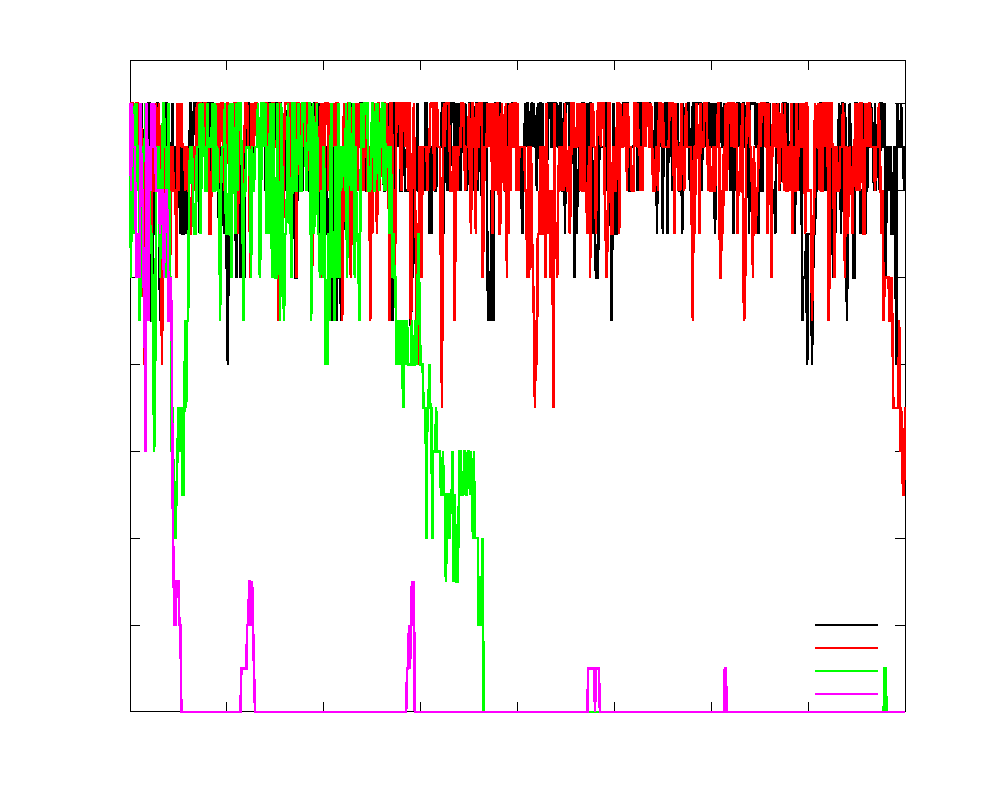
\includegraphics{images/data_knotts1/knotts1_lines}}%
    \gplfronttext
  \end{picture}%
\endgroup

                        \errorstopmode
                        \rule[-0.5cm]{0cm}{0cm}}

\caption{Basepair configuration (black: open, white: closed) for the 5'-GCGTCATACAGTGC-3' configuration of a B-DNA double helix (Knotts III.A.1, \cite{knotts2007coarse}) for different temperatures. Top-left: 330K; top-right: 335K; middle-left: 350K; middle-right:360K. Bottom: plot of number of closed basepairs for the time-evolution. The timescale on the x-axis is always in seconds (about 80 nanoseconds simulated).  } \label{knotts1_configs}\end{center}
\end{figure}

\paragraph{Knotts III.A.3: L60B36 Bubble Formation} This is a 60bp strand of dsDNA studied by, among others, Zeng \etal \cite{zeng}. The base sequence reads 5'-CCGCCAGCGG CGTTATTACATTTAATTCTTAAGTATTATAAGTAATATGGCCGCTGCGCC-3' and is designed to form a `bubble' at temperatures around the melting point because of the weaker base pairing for the Ab and Tb bases; with the stronger Cb and Gb bondings at the extrema of the strand. From the illustrations in Figure \ref{L60B36_configs} it is clear that the bubble formation exists and is the most clear between 340K and 350K, which agrees with the results of the simulations by Knotts \etal \cite{knotts2007coarse}.

\begin{figure}[hbt] \begin{minipage}{7cm}

               \scalebox{0.9}{
                        \nonstopmode
                        % GNUPLOT: LaTeX picture with Postscript
\begingroup
  \makeatletter
  \providecommand\color[2][]{%
    \GenericError{(gnuplot) \space\space\space\@spaces}{%
      Package color not loaded in conjunction with
      terminal option `colourtext'%
    }{See the gnuplot documentation for explanation.%
    }{Either use 'blacktext' in gnuplot or load the package
      color.sty in LaTeX.}%
    \renewcommand\color[2][]{}%
  }%
  \providecommand\includegraphics[2][]{%
    \GenericError{(gnuplot) \space\space\space\@spaces}{%
      Package graphicx or graphics not loaded%
    }{See the gnuplot documentation for explanation.%
    }{The gnuplot epslatex terminal needs graphicx.sty or graphics.sty.}%
    \renewcommand\includegraphics[2][]{}%
  }%
  \providecommand\rotatebox[2]{#2}%
  \@ifundefined{ifGPcolor}{%
    \newif\ifGPcolor
    \GPcolortrue
  }{}%
  \@ifundefined{ifGPblacktext}{%
    \newif\ifGPblacktext
    \GPblacktexttrue
  }{}%
  % define a \g@addto@macro without @ in the name:
  \let\gplgaddtomacro\g@addto@macro
  % define empty templates for all commands taking text:
  \gdef\gplbacktext{}%
  \gdef\gplfronttext{}%
  \makeatother
  \ifGPblacktext
    % no textcolor at all
    \def\colorrgb#1{}%
    \def\colorgray#1{}%
  \else
    % gray or color?
    \ifGPcolor
      \def\colorrgb#1{\color[rgb]{#1}}%
      \def\colorgray#1{\color[gray]{#1}}%
      \expandafter\def\csname LTw\endcsname{\color{white}}%
      \expandafter\def\csname LTb\endcsname{\color{black}}%
      \expandafter\def\csname LTa\endcsname{\color{black}}%
      \expandafter\def\csname LT0\endcsname{\color[rgb]{1,0,0}}%
      \expandafter\def\csname LT1\endcsname{\color[rgb]{0,1,0}}%
      \expandafter\def\csname LT2\endcsname{\color[rgb]{0,0,1}}%
      \expandafter\def\csname LT3\endcsname{\color[rgb]{1,0,1}}%
      \expandafter\def\csname LT4\endcsname{\color[rgb]{0,1,1}}%
      \expandafter\def\csname LT5\endcsname{\color[rgb]{1,1,0}}%
      \expandafter\def\csname LT6\endcsname{\color[rgb]{0,0,0}}%
      \expandafter\def\csname LT7\endcsname{\color[rgb]{1,0.3,0}}%
      \expandafter\def\csname LT8\endcsname{\color[rgb]{0.5,0.5,0.5}}%
    \else
      % gray
      \def\colorrgb#1{\color{black}}%
      \def\colorgray#1{\color[gray]{#1}}%
      \expandafter\def\csname LTw\endcsname{\color{white}}%
      \expandafter\def\csname LTb\endcsname{\color{black}}%
      \expandafter\def\csname LTa\endcsname{\color{black}}%
      \expandafter\def\csname LT0\endcsname{\color{black}}%
      \expandafter\def\csname LT1\endcsname{\color{black}}%
      \expandafter\def\csname LT2\endcsname{\color{black}}%
      \expandafter\def\csname LT3\endcsname{\color{black}}%
      \expandafter\def\csname LT4\endcsname{\color{black}}%
      \expandafter\def\csname LT5\endcsname{\color{black}}%
      \expandafter\def\csname LT6\endcsname{\color{black}}%
      \expandafter\def\csname LT7\endcsname{\color{black}}%
      \expandafter\def\csname LT8\endcsname{\color{black}}%
    \fi
  \fi
  \setlength{\unitlength}{0.0500bp}%
  \begin{picture}(5760.00,3840.00)%
    \gplgaddtomacro\gplfronttext{%
      \colorrgb{0.00,0.00,0.00}%
      \put(616,3074){\makebox(0,0)[r]{\strut{}10}}%
      \colorrgb{0.00,0.00,0.00}%
      \put(616,2543){\makebox(0,0)[r]{\strut{}20}}%
      \colorrgb{0.00,0.00,0.00}%
      \put(616,2013){\makebox(0,0)[r]{\strut{}30}}%
      \colorrgb{0.00,0.00,0.00}%
      \put(616,1483){\makebox(0,0)[r]{\strut{}40}}%
      \colorrgb{0.00,0.00,0.00}%
      \put(616,952){\makebox(0,0)[r]{\strut{}50}}%
      \colorrgb{0.00,0.00,0.00}%
      \put(616,422){\makebox(0,0)[r]{\strut{}60}}%
      \colorrgb{0.00,0.00,0.00}%
      \put(748,202){\makebox(0,0){\strut{}0}}%
      \colorrgb{0.00,0.00,0.00}%
      \put(1385,202){\makebox(0,0){\strut{}1e-08}}%
      \colorrgb{0.00,0.00,0.00}%
      \put(2022,202){\makebox(0,0){\strut{}2e-08}}%
      \colorrgb{0.00,0.00,0.00}%
      \put(2658,202){\makebox(0,0){\strut{}3e-08}}%
      \colorrgb{0.00,0.00,0.00}%
      \put(3295,202){\makebox(0,0){\strut{}4e-08}}%
      \colorrgb{0.00,0.00,0.00}%
      \put(3932,202){\makebox(0,0){\strut{}5e-08}}%
      \colorrgb{0.00,0.00,0.00}%
      \put(4569,202){\makebox(0,0){\strut{}6e-08}}%
      \colorrgb{0.00,0.00,0.00}%
      \put(5206,202){\makebox(0,0){\strut{}7e-08}}%
    }%
    \gplbacktext
    \put(0,0){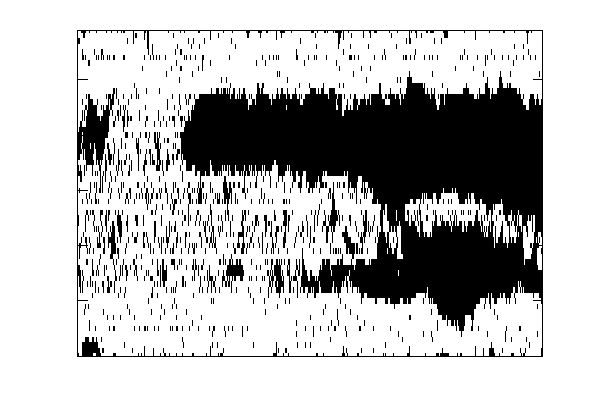
\includegraphics{images/data_L60B36_70ns/L60B36_70ns_T340}}%
    \gplfronttext
  \end{picture}%
\endgroup

                        \errorstopmode
                        \rule[-0.5cm]{0cm}{0cm}}

 \end{minipage} \begin{minipage}{7cm} -e \begin{figure}[htb]
       \begin{center}
               \scalebox{0.9}{
                        \nonstopmode
                        % GNUPLOT: LaTeX picture with Postscript
\begingroup
  \makeatletter
  \providecommand\color[2][]{%
    \GenericError{(gnuplot) \space\space\space\@spaces}{%
      Package color not loaded in conjunction with
      terminal option `colourtext'%
    }{See the gnuplot documentation for explanation.%
    }{Either use 'blacktext' in gnuplot or load the package
      color.sty in LaTeX.}%
    \renewcommand\color[2][]{}%
  }%
  \providecommand\includegraphics[2][]{%
    \GenericError{(gnuplot) \space\space\space\@spaces}{%
      Package graphicx or graphics not loaded%
    }{See the gnuplot documentation for explanation.%
    }{The gnuplot epslatex terminal needs graphicx.sty or graphics.sty.}%
    \renewcommand\includegraphics[2][]{}%
  }%
  \providecommand\rotatebox[2]{#2}%
  \@ifundefined{ifGPcolor}{%
    \newif\ifGPcolor
    \GPcolortrue
  }{}%
  \@ifundefined{ifGPblacktext}{%
    \newif\ifGPblacktext
    \GPblacktexttrue
  }{}%
  % define a \g@addto@macro without @ in the name:
  \let\gplgaddtomacro\g@addto@macro
  % define empty templates for all commands taking text:
  \gdef\gplbacktext{}%
  \gdef\gplfronttext{}%
  \makeatother
  \ifGPblacktext
    % no textcolor at all
    \def\colorrgb#1{}%
    \def\colorgray#1{}%
  \else
    % gray or color?
    \ifGPcolor
      \def\colorrgb#1{\color[rgb]{#1}}%
      \def\colorgray#1{\color[gray]{#1}}%
      \expandafter\def\csname LTw\endcsname{\color{white}}%
      \expandafter\def\csname LTb\endcsname{\color{black}}%
      \expandafter\def\csname LTa\endcsname{\color{black}}%
      \expandafter\def\csname LT0\endcsname{\color[rgb]{1,0,0}}%
      \expandafter\def\csname LT1\endcsname{\color[rgb]{0,1,0}}%
      \expandafter\def\csname LT2\endcsname{\color[rgb]{0,0,1}}%
      \expandafter\def\csname LT3\endcsname{\color[rgb]{1,0,1}}%
      \expandafter\def\csname LT4\endcsname{\color[rgb]{0,1,1}}%
      \expandafter\def\csname LT5\endcsname{\color[rgb]{1,1,0}}%
      \expandafter\def\csname LT6\endcsname{\color[rgb]{0,0,0}}%
      \expandafter\def\csname LT7\endcsname{\color[rgb]{1,0.3,0}}%
      \expandafter\def\csname LT8\endcsname{\color[rgb]{0.5,0.5,0.5}}%
    \else
      % gray
      \def\colorrgb#1{\color{black}}%
      \def\colorgray#1{\color[gray]{#1}}%
      \expandafter\def\csname LTw\endcsname{\color{white}}%
      \expandafter\def\csname LTb\endcsname{\color{black}}%
      \expandafter\def\csname LTa\endcsname{\color{black}}%
      \expandafter\def\csname LT0\endcsname{\color{black}}%
      \expandafter\def\csname LT1\endcsname{\color{black}}%
      \expandafter\def\csname LT2\endcsname{\color{black}}%
      \expandafter\def\csname LT3\endcsname{\color{black}}%
      \expandafter\def\csname LT4\endcsname{\color{black}}%
      \expandafter\def\csname LT5\endcsname{\color{black}}%
      \expandafter\def\csname LT6\endcsname{\color{black}}%
      \expandafter\def\csname LT7\endcsname{\color{black}}%
      \expandafter\def\csname LT8\endcsname{\color{black}}%
    \fi
  \fi
  \setlength{\unitlength}{0.0500bp}%
  \begin{picture}(5760.00,3840.00)%
    \gplgaddtomacro\gplbacktext{%
      \colorrgb{0.00,0.00,0.00}%
      \put(110,1986){\rotatebox{90}{\makebox(0,0){\strut{}\rule{0pt}{-1.5cm}Basepair configuration}}}%
      \colorrgb{0.00,0.00,0.00}%
      \put(2980,-128){\makebox(0,0){\strut{}Time (seconds)}}%
    }%
    \gplgaddtomacro\gplfronttext{%
      \colorrgb{0.00,0.00,0.00}%
      \put(616,3074){\makebox(0,0)[r]{\strut{}10}}%
      \colorrgb{0.00,0.00,0.00}%
      \put(616,2543){\makebox(0,0)[r]{\strut{}20}}%
      \colorrgb{0.00,0.00,0.00}%
      \put(616,2013){\makebox(0,0)[r]{\strut{}30}}%
      \colorrgb{0.00,0.00,0.00}%
      \put(616,1483){\makebox(0,0)[r]{\strut{}40}}%
      \colorrgb{0.00,0.00,0.00}%
      \put(616,952){\makebox(0,0)[r]{\strut{}50}}%
      \colorrgb{0.00,0.00,0.00}%
      \put(616,422){\makebox(0,0)[r]{\strut{}60}}%
      \colorrgb{0.00,0.00,0.00}%
      \put(748,202){\makebox(0,0){\strut{}0}}%
      \colorrgb{0.00,0.00,0.00}%
      \put(1385,202){\makebox(0,0){\strut{}1e-08}}%
      \colorrgb{0.00,0.00,0.00}%
      \put(2022,202){\makebox(0,0){\strut{}2e-08}}%
      \colorrgb{0.00,0.00,0.00}%
      \put(2658,202){\makebox(0,0){\strut{}3e-08}}%
      \colorrgb{0.00,0.00,0.00}%
      \put(3295,202){\makebox(0,0){\strut{}4e-08}}%
      \colorrgb{0.00,0.00,0.00}%
      \put(3932,202){\makebox(0,0){\strut{}5e-08}}%
      \colorrgb{0.00,0.00,0.00}%
      \put(4569,202){\makebox(0,0){\strut{}6e-08}}%
      \colorrgb{0.00,0.00,0.00}%
      \put(5206,202){\makebox(0,0){\strut{}7e-08}}%
    }%
    \gplbacktext
    \put(0,0){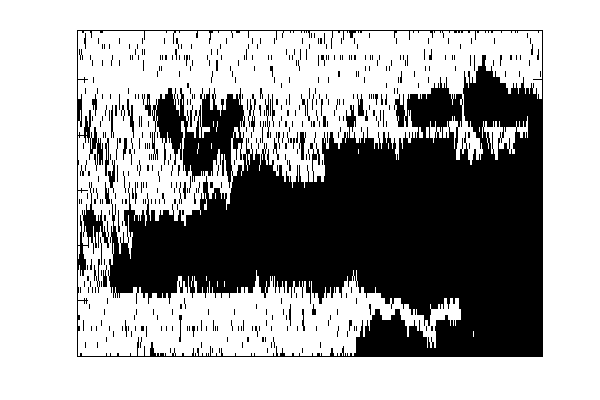
\includegraphics{images/data_L60B36_70ns/L60B36_70ns_T350}}%
    \gplfronttext
  \end{picture}%
\endgroup

                        \errorstopmode
                        \rule[-0.5cm]{0cm}{0cm}}
                \caption{}
        \end{center}
\end{figure}

 \end{minipage}
\begin{minipage}{8cm}

               \scalebox{0.9}{
                        \nonstopmode
                        % GNUPLOT: LaTeX picture with Postscript
\begingroup
  \makeatletter
  \providecommand\color[2][]{%
    \GenericError{(gnuplot) \space\space\space\@spaces}{%
      Package color not loaded in conjunction with
      terminal option `colourtext'%
    }{See the gnuplot documentation for explanation.%
    }{Either use 'blacktext' in gnuplot or load the package
      color.sty in LaTeX.}%
    \renewcommand\color[2][]{}%
  }%
  \providecommand\includegraphics[2][]{%
    \GenericError{(gnuplot) \space\space\space\@spaces}{%
      Package graphicx or graphics not loaded%
    }{See the gnuplot documentation for explanation.%
    }{The gnuplot epslatex terminal needs graphicx.sty or graphics.sty.}%
    \renewcommand\includegraphics[2][]{}%
  }%
  \providecommand\rotatebox[2]{#2}%
  \@ifundefined{ifGPcolor}{%
    \newif\ifGPcolor
    \GPcolortrue
  }{}%
  \@ifundefined{ifGPblacktext}{%
    \newif\ifGPblacktext
    \GPblacktexttrue
  }{}%
  % define a \g@addto@macro without @ in the name:
  \let\gplgaddtomacro\g@addto@macro
  % define empty templates for all commands taking text:
  \gdef\gplbacktext{}%
  \gdef\gplfronttext{}%
  \makeatother
  \ifGPblacktext
    % no textcolor at all
    \def\colorrgb#1{}%
    \def\colorgray#1{}%
  \else
    % gray or color?
    \ifGPcolor
      \def\colorrgb#1{\color[rgb]{#1}}%
      \def\colorgray#1{\color[gray]{#1}}%
      \expandafter\def\csname LTw\endcsname{\color{white}}%
      \expandafter\def\csname LTb\endcsname{\color{black}}%
      \expandafter\def\csname LTa\endcsname{\color{black}}%
      \expandafter\def\csname LT0\endcsname{\color[rgb]{1,0,0}}%
      \expandafter\def\csname LT1\endcsname{\color[rgb]{0,1,0}}%
      \expandafter\def\csname LT2\endcsname{\color[rgb]{0,0,1}}%
      \expandafter\def\csname LT3\endcsname{\color[rgb]{1,0,1}}%
      \expandafter\def\csname LT4\endcsname{\color[rgb]{0,1,1}}%
      \expandafter\def\csname LT5\endcsname{\color[rgb]{1,1,0}}%
      \expandafter\def\csname LT6\endcsname{\color[rgb]{0,0,0}}%
      \expandafter\def\csname LT7\endcsname{\color[rgb]{1,0.3,0}}%
      \expandafter\def\csname LT8\endcsname{\color[rgb]{0.5,0.5,0.5}}%
    \else
      % gray
      \def\colorrgb#1{\color{black}}%
      \def\colorgray#1{\color[gray]{#1}}%
      \expandafter\def\csname LTw\endcsname{\color{white}}%
      \expandafter\def\csname LTb\endcsname{\color{black}}%
      \expandafter\def\csname LTa\endcsname{\color{black}}%
      \expandafter\def\csname LT0\endcsname{\color{black}}%
      \expandafter\def\csname LT1\endcsname{\color{black}}%
      \expandafter\def\csname LT2\endcsname{\color{black}}%
      \expandafter\def\csname LT3\endcsname{\color{black}}%
      \expandafter\def\csname LT4\endcsname{\color{black}}%
      \expandafter\def\csname LT5\endcsname{\color{black}}%
      \expandafter\def\csname LT6\endcsname{\color{black}}%
      \expandafter\def\csname LT7\endcsname{\color{black}}%
      \expandafter\def\csname LT8\endcsname{\color{black}}%
    \fi
  \fi
  \setlength{\unitlength}{0.0500bp}%
  \begin{picture}(5760.00,3840.00)%
    \gplgaddtomacro\gplbacktext{%
      \colorrgb{0.00,0.00,0.00}%
      \put(110,1986){\rotatebox{90}{\makebox(0,0){\strut{}\rule{0pt}{-1.5cm}Basepair configuration}}}%
      \colorrgb{0.00,0.00,0.00}%
      \put(2980,-128){\makebox(0,0){\strut{}Time (seconds)}}%
    }%
    \gplgaddtomacro\gplfronttext{%
      \colorrgb{0.00,0.00,0.00}%
      \put(616,3074){\makebox(0,0)[r]{\strut{}10}}%
      \colorrgb{0.00,0.00,0.00}%
      \put(616,2543){\makebox(0,0)[r]{\strut{}20}}%
      \colorrgb{0.00,0.00,0.00}%
      \put(616,2013){\makebox(0,0)[r]{\strut{}30}}%
      \colorrgb{0.00,0.00,0.00}%
      \put(616,1483){\makebox(0,0)[r]{\strut{}40}}%
      \colorrgb{0.00,0.00,0.00}%
      \put(616,952){\makebox(0,0)[r]{\strut{}50}}%
      \colorrgb{0.00,0.00,0.00}%
      \put(616,422){\makebox(0,0)[r]{\strut{}60}}%
      \colorrgb{0.00,0.00,0.00}%
      \put(748,202){\makebox(0,0){\strut{}0}}%
      \colorrgb{0.00,0.00,0.00}%
      \put(1385,202){\makebox(0,0){\strut{}1e-08}}%
      \colorrgb{0.00,0.00,0.00}%
      \put(2022,202){\makebox(0,0){\strut{}2e-08}}%
      \colorrgb{0.00,0.00,0.00}%
      \put(2658,202){\makebox(0,0){\strut{}3e-08}}%
      \colorrgb{0.00,0.00,0.00}%
      \put(3295,202){\makebox(0,0){\strut{}4e-08}}%
      \colorrgb{0.00,0.00,0.00}%
      \put(3932,202){\makebox(0,0){\strut{}5e-08}}%
      \colorrgb{0.00,0.00,0.00}%
      \put(4569,202){\makebox(0,0){\strut{}6e-08}}%
      \colorrgb{0.00,0.00,0.00}%
      \put(5206,202){\makebox(0,0){\strut{}7e-08}}%
    }%
    \gplbacktext
    \put(0,0){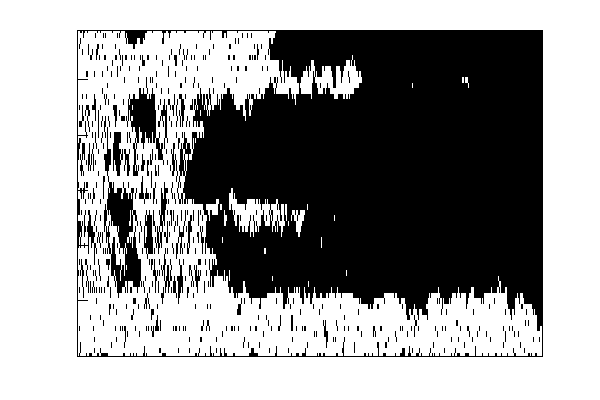
\includegraphics{images/data_L60B36_70ns/L60B36_70ns_T360}}%
    \gplfronttext
  \end{picture}%
\endgroup

                        \errorstopmode
                        \rule[-0.5cm]{0cm}{0cm}}


 \end{minipage} \begin{minipage}{6cm}
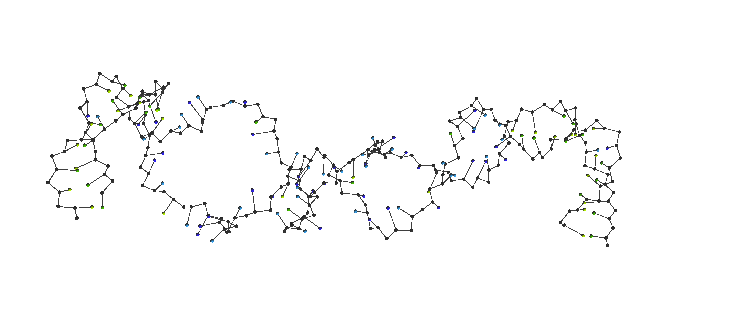
\includegraphics[width=7cm]{images/L60B36_bubble2.png}\\
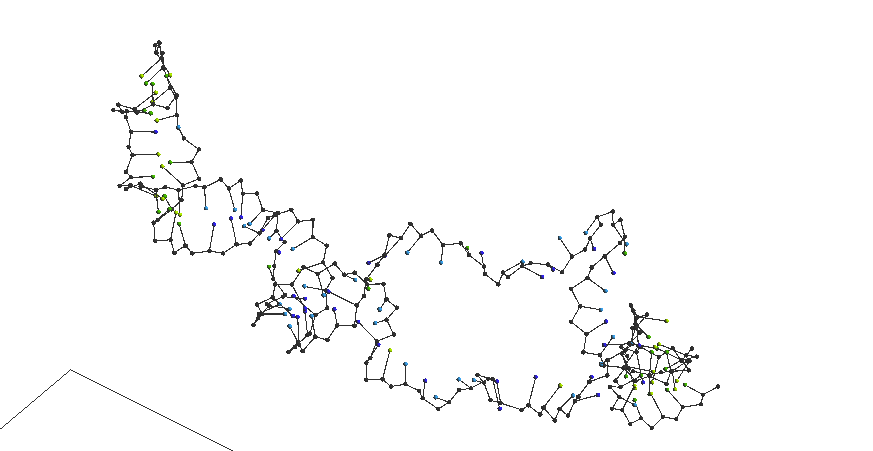
\includegraphics[width=7cm]{images/L60B36_bubble1.png} \end{minipage}
\begin{center}
\caption{Basepairing configuration (y-axis) for bubble formation in the L60B36 dsDNA configuration (white: closed basepairs, black: open basepairs) for a time-evolution of 80 nanoseconds (x-axis) at 340K (top-left), 350K (top-right) and 360K (bottom-left). The process of bubble formation is illustrated in two bubble configurations at 340K (bottom-right panel, top configuration) and at 350K (bottom configuration). }\label{L60B36_configs}
\end{center}
\end{figure}

The characteristic time of the unwinding process of double stranded DNA in function of the polymer length has been predicted numerous times with numerous simulation techniques. Baiesi, Barkema, Carlon \& Panja \cite{carlon2010unwinding} used Monte Carlo methods to determine that the time needed to unwind a double stranded polymer of length $N$ in a wound structure (yielding a basic simulation of the global dynamics of the unwinding process) goes like
\begin{equation}
\tau \sim N^{2.57\pm 0.03}.
\end{equation}
Later work by Walter, Ferrantini, Carlon \& Vanderzande \cite{walter2011fractional} pushed this coeffici\"ent down to 
\begin{equation}
\tau \sim N^{2.26 \pm 0.02}
\end{equation}
when incorporating a slightly more complicated dynamics. Both papers also point out that modeling DNA denaturation as an equilibrium process yields time scaling laws much closer to the linear case.


\subsection{Hairpin formation}

\begin{figure}[hbt]
\begin{center}
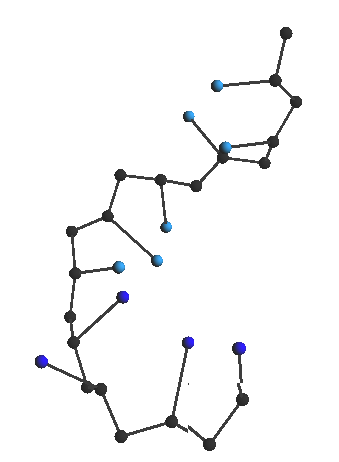
\includegraphics[width=4cm]{images/results_hairpin1}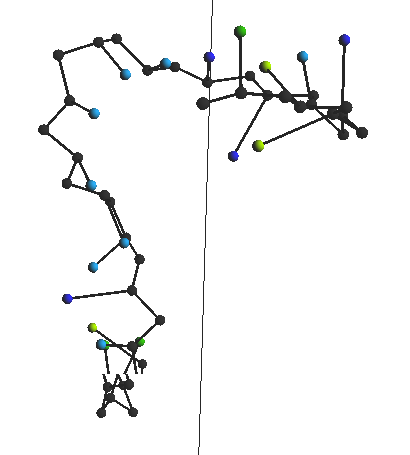
\includegraphics[width=5cm]{images/results_hairpin2}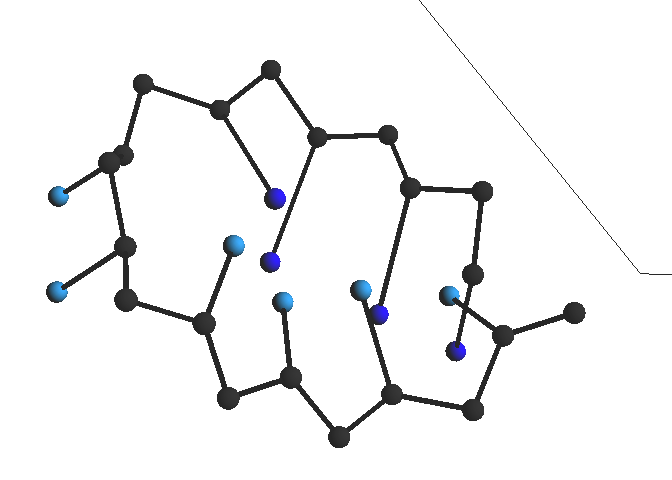
\includegraphics[width=5cm]{images/results_hairpin3}
\end{center}
\caption{Stages of hairpin formation of a single strand with a stemlength of 7 basepairs and a loopsize of 4 monomers (5'-GCCTATTTTTTAATAGGC-3'). This hairpin was formed after $\sim$ 50ns simulation time at 290K and salt concentration 100 mM.}
\label{results_hairpin}
\end{figure}





